\chapter{РЕАЛИЗАЦИЯ ПРОГРАММНОЙ СИСТЕМЫ}

\section{Реализация логики игры}

Базовый класс \texttt{SnakeGame} отвечает за основную механику игры. В нём реализованы положение головы и тела змейки, проверка столкновений, рост длины после поедания пищи и выбор свободной клетки для новой еды.

Также в игре есть защита от мгновенного разворота на 180 градусов. Это соответствует обычным правилам <<Змейки>> и убирает некорректные переходы между состояниями.

Такое разделение полезно тем, что игровая логика остаётся независимой от обучения. Игра умеет корректно работать сама по себе: обновлять положение объектов, проверять конец партии и поддерживать состояние поля. Благодаря этому один и тот же игровой движок можно использовать и для ручного режима, и для обучения, и для наблюдения за уже обученным агентом.

\section{Реализация RL-среды и Q-learning агента}

Среда переводит игровую механику в форму, удобную для обучения. По текущему положению змейки строится вектор состояния, затем принимается одно из трёх действий, после чего среда возвращает награду, новое состояние и признак завершения эпизода.

Класс \texttt{QLearningAgent} хранит Q-таблицу в виде словаря. Ключом служит кортеж признаков состояния, а значением --- список оценок для трёх действий. Если состояние встречается впервые, для него создаётся набор нулевых оценок.

Выбор действия строится по $\varepsilon$-жадному правилу: иногда агент делает случайный ход, а иногда выбирает лучший из уже известных. После каждого шага вызывается функция \texttt{update}, которая обновляет Q-значение для пары <<состояние --- действие>>.

Если рассмотреть один эпизод обучения по шагам, то процесс выглядит так. Сначала среда возвращает текущее состояние. Затем агент по этому состоянию выбирает действие. После выполнения действия игра переходит в новую конфигурацию, а среда вычисляет награду. Далее агент получает новое состояние и обновляет соответствующее значение в Q-таблице. Такой цикл повторяется до тех пор, пока змейка не столкнётся с препятствием или не завершится текущая партия.

Преимущество такой схемы в том, что она хорошо согласуется с формальной моделью reinforcement learning. Каждый шаг обучения можно описать как переход из одного состояния в другое с фиксированным действием и численной наградой. Это делает программу не просто игровой реализацией, а полноценной учебной RL-средой.

\section{Реализация интерфейса и режимов работы программы}

Визуальная часть сделана на библиотеке \texttt{pygame}. Программа рисует поле, еду, змейку, строку состояния и окно завершения игры. Также есть ручной режим и режим наблюдения за уже обученным агентом \cite{matthes2023python,pygame_docs}.

\begin{figure}[H]
    \centering
    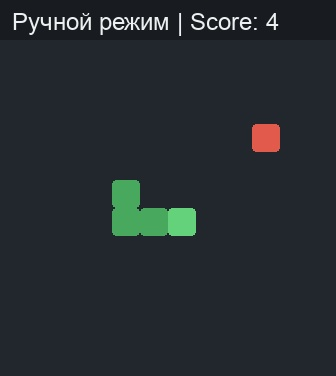
\includegraphics[width=0.42\textwidth]{images/manual_game.jpg}
    \caption{Интерфейс программы в режиме ручной игры}
\end{figure}

\begin{figure}[H]
    \centering
    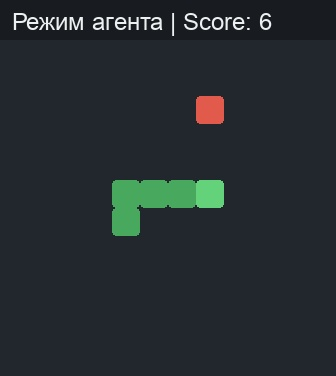
\includegraphics[width=0.42\textwidth]{images/agent_mode.jpg}
    \caption{Интерфейс программы в режиме наблюдения за агентом}
\end{figure}

\begin{figure}[H]
    \centering
    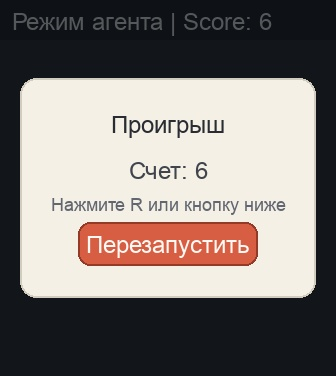
\includegraphics[width=0.42\textwidth]{images/game_over_modal.jpg}
    \caption{Модальное окно завершения партии и перезапуска}
\end{figure}

\section{Сохранение обученной политики и структура модулей}

После обучения таблица сохраняется в файл \texttt{artifacts/q\_table.pkl}. Благодаря этому можно запускать агента в режиме \texttt{watch} без повторного обучения. Это удобно и для экспериментов, и для демонстрации работы программы.

Практическая ценность сохранения Q-таблицы состоит в том, что обучение и демонстрация результатов становятся независимыми друг от друга. Не нужно каждый раз заново запускать длинную процедуру обучения, чтобы показать поведение агента. Можно один раз получить таблицу, а затем использовать её для серии визуальных запусков, сравнения поведения в разных ситуациях и подготовки иллюстраций для отчёта.

С точки зрения структуры проекта это решение также полезно тем, что отделяет этап накопления опыта от этапа использования уже готовой стратегии. Такая схема особенно удобна для курсовой работы: она позволяет сначала описать процесс обучения как вычислительный эксперимент, а затем отдельно показать практический результат в виде наблюдаемого игрового поведения.

\begin{table}[H]
    \centering
    \caption{Назначение основных модулей проекта}
    \begin{tabularx}{\textwidth}{>{\raggedright\arraybackslash}p{0.22\textwidth} X}
        \toprule
        Файл & Назначение \\
        \midrule
        \texttt{main.py} & Разбор аргументов командной строки и переключение режимов \texttt{play/train/watch} \\
        \texttt{train.py} & Создание среды и агента, организация эпизодов обучения, вычисление итоговых метрик \\
        \texttt{agent.py} & Хранение Q-таблицы, $\varepsilon$-жадный выбор действий, обновление оценок, сохранение и загрузка \\
        \texttt{env.py} & Преобразование игры в RL-среду с вектором состояния и системой наград \\
        \texttt{game.py} & Низкоуровневая логика игры, проверка столкновений и генерация пищи \\
        \texttt{render.py} & Визуализация, ручное управление, режим наблюдения за агентом \\
        \texttt{tests/} & Набор автоматических тестов для проверки основных компонентов \\
        \bottomrule
    \end{tabularx}
\end{table}

Каждый из этих модулей выполняет самостоятельную роль, но максимальный эффект они дают именно в связке. Игровой модуль формирует динамику среды, среда переводит её в RL-формат, агент учится на переходах, модуль обучения организует серию эпизодов, а визуализация позволяет наглядно увидеть итог поведения. Благодаря этому проект выглядит как завершённая система, а не как набор разрозненных программных фрагментов.
